% printing information at UW-Madison: https://designlab.wisc.edu/resources/projects/posters/

\PassOptionsToPackage{dvipsnames}{xcolor}
\documentclass[final]{beamer}

\usepackage[T1]{fontenc}
\usepackage{lmodern}

% set poster dimensions below (in cm)
% AFI / the posterboards at the Discovery Building are 46"x46".
% 46" wide x 36" high (121.92 x 91.44 cm)
% A0 for ASA WI Chapter, which is slightly smaller 84.1 x 118.9 (46.8 wide by 33.1 tall)
% \usepackage[orientation=landscape, size=a0, scale=1]{beamerposter}

% A0 margins + 0.5 cm bleed in each direction?
\usepackage[orientation=landscape,width=119.9cm,height=85.1cm, scale=1]{beamerposter}

% https://mirror.math.princeton.edu/pub/CTAN/macros/latex/contrib/crop/crop.pdf
% \usepackage[width=119.9cm,height=85.1cm,noaxes,frame,lualatex,landscape,center]{crop}

% \usepackage{geometry}

\usetheme{gemini}
\usecolortheme{mit}
\usepackage{graphicx}
\usepackage{tikz}
\usepackage{xcolor}
\usepackage{nicematrix}

\usepackage[backend=bibtex, sortcites, style=authoryear]{biblatex}
\addbibresource{references.bib}

% https://tex.stackexchange.com/questions/585635/beamer-biblatex-authoryear-causes-problem-with-insertbiblabel
\setbeamertemplate{bibliography item}{}

\usepackage{tikz}
\usepackage[protrusion=true,expansion=true]{microtype}
\usepackage{anyfontsize}
\usepackage{hyperref}
\usepackage{amsmath}

\newcommand{\Ni}{\mathcal N(i)}
\newcommand{\R}{\mathbb{R}}
\newcommand{\alphahat}{\hat{\alpha}}
\newcommand{\gammahat}{\hat{\gamma}}
\newcommand{\deltahat}{\hat{\delta}}
\newcommand{\betahat}{\hat{\beta}}
\newcommand \Omegap [1] {\Omega_P \left(#1\right)}
\DeclareMathOperator*{\supp}{supp}

% If you have N columns, choose \sepwidth and \colwidth such that
% (N+1)*\sepwidth + N*\colwidth = \paperwidth
\newlength{\sepwidth}
\newlength{\colwidth}
\setlength{\sepwidth}{0.025\paperwidth}
\setlength{\colwidth}{0.3\paperwidth}

\newcommand{\separatorcolumn}{\begin{column}{\sepwidth}\end{column}}

\title{Estimating peer influence: limitations of linear-in-means models}
\author{Alex Hayes \inst{1} \and Keith Levin \inst{1}}
\institute[shortinst]{\inst{1} Department of Statistics, University of Wisconsin-Madison}
\logoright{
\includegraphics[height=7cm]{figures/logos/color-flush-UWlogo-print.pdf}}
% \footercontent{\hfill \href{https://www.alexpghayes.com}{https://www.alexpghayes.com}}

\begin{document}

\begin{frame}[t]
    \begin{columns}[t]
        \separatorcolumn

        \begin{column}{\colwidth}

            \begin{block}{Understanding social influence is a fundamental problem in a highly connected society}

                \vspace{4mm}

                \begin{minipage}{.25\textwidth}
                    \centering
                    \begin{tikzpicture}
                        \node[shape=circle,fill=Mahogany] (A) at (0,1) {};
                        \node[shape=circle,fill=gray,label=below left:{
\includegraphics[scale=0.4]{./figures/bacteria.png}}] (B) at (1,-1) {};
                        \node[shape=circle,fill=Mahogany] (C) at (1.5,2.5) {};
                        \node[shape=circle,fill=Mahogany] (D) at (2.75,0.5) {};
                        \node[shape=circle,fill=gray,label=above right:{
\includegraphics[scale=0.4]{./figures/bacteria.png}}] (E) at (4.3,2.4) {};
                        \node[shape=circle,fill=Mahogany,label=below:{
\includegraphics[scale=0.4]{./figures/bacteria.png}}] (F) at (3.4,-1.4) {};
                        \node[shape=circle,fill=gray,label=right:{
\includegraphics[scale=0.4]{./figures/bacteria.png}}] (G) at (4.7,0.1) {};

                        \draw (A) -- (B);
                        \draw (A) -- (C);
                        \draw (B) -- (C);
                        \draw (B) -- (D) -- (F);
                        \draw (C) -- (D) -- (E);
                        \draw (B) -- (F) -- (G) -- (E) -- (C);
                    \end{tikzpicture}
                \end{minipage}
                \begin{minipage}{.75\textwidth}
                    \vspace{7mm}
                    \textbf{Direct effect}: if I get \textcolor{Mahogany}{vaccinated}, I am less likely to get sick 
\includegraphics[scale=0.4]{./figures/bacteria.png}
                    \vspace{6mm} \\
                    \textbf{Contagion}: if my friends get sick 
\includegraphics[scale=0.4]{./figures/bacteria.png}, I am more likely to get sick 
\includegraphics[scale=0.4]{./figures/bacteria.png}
                    \vspace{6mm} \\
                    \textbf{Interference}: if my friends get \textcolor{Mahogany}{vaccinated}, I am less likely to get sick 
\includegraphics[scale=0.4]{./figures/bacteria.png}
                \end{minipage}
            \end{block}

            \begin{block}{The linear-in-means model is a canonical tool to estimate peer influence in network data}
                \begin{equation*}
                    \underbrace{Y_i}_\text{sick?} =
                    \alpha +
                    \beta \underbrace{\frac{1}{d_i}\sum_{j \in \Ni} Y_j}_{\substack{\text{fraction} \\ \text{sick} \\ \text{friends}}} +
                    \gamma \, T_i +
                    \delta \underbrace{\frac{1}{d_i}\sum_{j \in \Ni} T_j}_{\substack{\text{fraction} \\ \text{vaccinated} \\ \text{friends}}} + \,
                    \varepsilon_i
                \end{equation*}

                \begin{minipage}{.5\textwidth}
                    \textbf{Data:}
                    \vspace{3mm}
                    \begin{table}[]
                        \begin{tabular}{llcl}
                            Outcome         & (sick?)       & $Y_i$    & $\in \{0, 1\}$           \\
                            Treatment       & (vaccinated?) & $T_i$    & $\in \{0, 1\}$           \\
                            Edge $i \sim j$ & (friends?)    & $A_{ij}$ & $\in \{0, 1\}$           \\
                            Degree          & (num friends) & $d_i$    & $\in \{0, 1, 2, \dots\}$
                        \end{tabular}
                    \end{table}
                \end{minipage}
                \begin{minipage}{.5\textwidth}
                    \textbf{Parameters:}
                    \vspace{3mm}
                    \begin{table}[]
                        \begin{tabular}{lcl}
                            Base rate     & $\alpha$ & $\in \R$      \\
                            Contagion     & $\beta$  & $\in (-1, 1)$ \\
                            Direct effect & $\gamma$ & $\in \R$      \\
                            Interference  & $\delta$ & $\in \R$
                        \end{tabular}
                    \end{table}
                \end{minipage}

                Letting $G = D^{-1} A$ be the row-normalized adjacency matrix, can express in matrix-vector form:
                \begin{equation*} \label{eq:lim-mv}
                    Y = \alpha 1_n + \beta G Y + T \gamma + G T \delta + \varepsilon
                \end{equation*}
            \end{block}

            \begin{block}{Linear-in-means models are famously suspectible to the ``reflection problem,'' an identification failure due to colinearity}

                In highly structured networks, the peer effect terms can be perfectly colinear, such that peer effects cannot be estimated from the data. For example, in a fully connected network:

                \begin{figure}
                    \begin{minipage}{0.49\textwidth}
                        \centering
                        \begin{tikzpicture}
                            \node[shape=circle,fill=Mahogany,label=above left:{$T_1 = 1$}] (A) at (0,1) {};
                            \node[shape=circle,fill=gray,label=below left:{$T_2 = 0$}] (B) at (1,0) {};
                            \node[shape=circle,fill=Mahogany,label=above right:{$T_3 = 1$}] (C) at (1.5,1.5) {};
                            \node[shape=circle,fill=Mahogany,label=above right:{$T_4 = 1$}] (D) at (2.75,0.5) {};

                            \path (A) edge [loop above] node {} (A);
                            \path (B) edge [loop below] node {} (B);
                            \path (C) edge [loop above] node {} (C);
                            \path (D) edge [loop above] node {} (D);

                            \draw (A) -- (B);
                            \draw (A) -- (C);
                            \draw (A) -- (D);
                            \draw (B) -- (C);
                            \draw (B) -- (D);
                            \draw (C) -- (D);
                        \end{tikzpicture}
                    \end{minipage}
                    \begin{minipage}{0.49\textwidth}
                        \centering
                        \begin{tikzpicture}
                            \node[shape=circle,fill=Mahogany,label=above left:{$[GT]_1 = 3/4$}] (A) at (0,1) {};
                            \node[shape=circle,fill=gray,label=below left:{$[GT]_2 = 3/4$}] (B) at (1,0) {};
                            \node[shape=circle,fill=Mahogany,label=above right:{$[GT]_3 = 3/4$}] (C) at (1.5,1.5) {};
                            \node[shape=circle,fill=Mahogany,label=above right:{$[GT]_4 = 3/4$}] (D) at (2.75,0.5) {};

                            \path (A) edge [loop above] node {} (A);
                            \path (B) edge [loop below] node {} (B);
                            \path (C) edge [loop above] node {} (C);
                            \path (D) edge [loop above] node {} (D);

                            \draw (A) -- (B);
                            \draw (A) -- (C);
                            \draw (A) -- (D);
                            \draw (B) -- (C);
                            \draw (B) -- (D);
                            \draw (C) -- (D);
                        \end{tikzpicture}
                    \end{minipage}
                \end{figure}

                \begin{equation*}
                    \begin{bmatrix}
                        Y_1 \\
                        Y_2 \\
                        Y_3 \\
                        Y_4
                    \end{bmatrix}
                    =
                    \begin{bNiceMatrix}[first-row,first-col]
                         &                         &      &   &                           \\
                         & \textcolor{Mahogany}{1} & GY_1 & 1 & \textcolor{Mahogany}{3/4} \\
                         & \textcolor{Mahogany}{1} & GY_2 & 0 & \textcolor{Mahogany}{3/4} \\
                         & \textcolor{Mahogany}{1} & GY_3 & 1 & \textcolor{Mahogany}{3/4} \\
                         & \textcolor{Mahogany}{1} & GY_4 & 1 & \textcolor{Mahogany}{3/4} \\
                    \end{bNiceMatrix}
                    \begin{bmatrix}
                        \textcolor{Mahogany}{\alpha} \\
                        \beta                        \\
                        \gamma                       \\
                        \textcolor{Mahogany}{\delta}
                    \end{bmatrix}
                    +
                    \begin{bmatrix}
                        \varepsilon_1 \\
                        \varepsilon_2 \\
                        \varepsilon_3 \\
                        \varepsilon_4
                    \end{bmatrix}
                \end{equation*}

                Can't distinguish base rate $\textcolor{Mahogany}{\alpha}$ from interference $\textcolor{Mahogany}{\delta}$ due to colinearity. The measurement of the base rate and the fraction of vaccinated friends effects are rescaled versions of one another--it's impossible to differentiate between them.
            \end{block}
            \begin{block}{It's widely believed that colinearity problems can be avoided when certain identifying conditions, such as intransitivity, hold}

                \textbf{Proposition:}
                Suppose $\mathbb E[\varepsilon \mid T] = 0$ and that $|\beta| < 1$ and $\gamma \beta + \delta \neq 0$. For any fixed $n$, if $I, G$ and $G^2$ are linearly independent (i.e., $a I + b G + c G^2 = 0$ only if $a = b = c = 0$), then $\alpha, \beta, \gamma$ and $\delta$ are identified. If $I, G$ and $G^2$ are linearly dependent and no node is isolated, then $(\alpha, \beta, \gamma, \delta)$ are not identified.

                \textbf{Intuition}: Peer influence is identified when there are \textcolor{Mahogany}{open triangles} (``intransitivity'') in the network
                \vspace{8mm}
                \begin{columns}
                    \begin{column}{0.5\textwidth}
                        \centering
                        \begin{tikzpicture}
                            \node[shape=circle,fill=gray,label=above left:A] (A) at (0,1) {};
                            \node[shape=circle,fill=Mahogany,label=below left:B] (B) at (1,0) {};
                            \node[shape=circle,fill=Mahogany,label=above right:C] (C) at (1.5,1.5) {};
                            \node[shape=circle,fill=Mahogany,label=above right:D] (D) at (2.75,0.5) {};
                            \draw (A) -- (B);
                            \draw (A) -- (C);
                            \draw (B) -- (C);
                            \draw (C) -- (D);
                        \end{tikzpicture}
                    \end{column}
                    \begin{column}{0.5\textwidth}
                        \centering
                        Open: \textcolor{Mahogany}{$B \leftrightarrow C \leftrightarrow D \nleftrightarrow B$} \\
                        Closed: $A \leftrightarrow B \leftrightarrow C \leftrightarrow A$
                    \end{column}
                \end{columns}
            \end{block}

        \end{column}

        \separatorcolumn

        \begin{column}{\colwidth}


            \begin{block}{We show that peer effects can be inestimable even when identifying conditions hold}
                Three popular estimators all fail to estimate parameters at expected $\sqrt{n}$ rates in simulations, even though half of all possible triangles in the network are open
                \begin{figure}
                    \centering
                    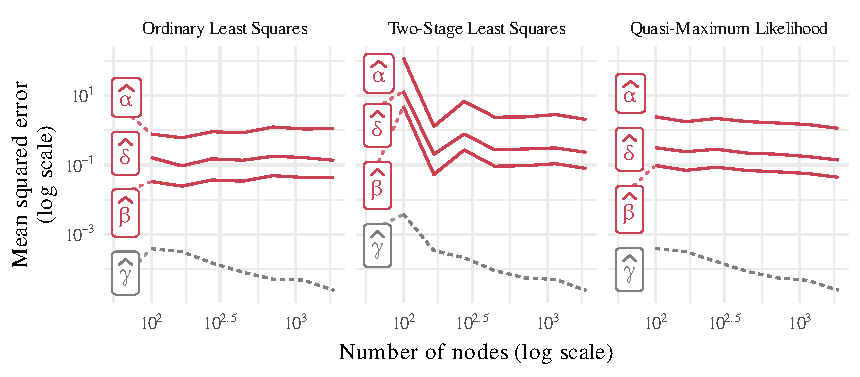
\includegraphics[width=0.9\textwidth]{./figures/simulations/biometrika-mse.pdf}
                \end{figure}
            \end{block}

            \begin{block}{The problem is that peer effect terms become more and more colinear as the number of nodes in the network increases}

                \textbf{Intuition:} Imagine vaccination is a coin flip for every node (i.e., a Bernoulli design). As the network grows, the fraction of vaccinated friends $\approx 0.5$ for every single node.

                \begin{equation} \label{eq:avg}
                    \lim_{d_i \to \infty}
                    \underbrace{[GT]_i}_{\substack{\text{fraction} \\ \text{vaccinated} \\ \text{friends}}}
                    =
                    \lim_{d_i \to \infty}
                    \underbrace{
                        \frac{1}{d_i} \sum_{j \in \Ni} T_j
                    }_{\substack{\text{average of $d_i$}           \\ \text{i.i.d. coin flips}}}
                    = \frac 12
                \end{equation}
                This also causes the contagion term to be near-colinear with the intercept, since $GY$ is a repeated diffusion of $T$ and $GT$ over the network
                \begin{align*}
                    Y & = \alpha 1_n + \beta G Y + \gamma T + \delta G T + \varepsilon                                \\
                      & = \left(I - \beta G\right)^{-1} \left(\alpha 1_n + \gamma T + \delta G T + \varepsilon\right) \\
                      & = \sum_{k=0}^\infty \beta^k G^k \left(\alpha 1_n + \gamma T + \delta G T + \varepsilon\right)
                \end{align*}

                \textbf{Lemma:} Suppose that (1) the nodal covariates $T_1, T_2, \dots$ are independent with shared mean $\tau \in \R$, and $T$ is independent of $A$; (2) the nodal covariates are sub-gamma random variables; (3) the regression errors $\varepsilon_1, \varepsilon_2, \dots$ are independent subgamma random variables independent of $T$.

                If the minimum degree of the network grows at a $\omega(\log n)$ rate, then there exists $\eta \in \R$ such that
                \begin{equation*}
                    \max_{i \in [n]} \Big| [GT]_i - \tau \Big|
                    = o(1) ~ \text{ and }
                    \max_{i \in [n]} \Big| [GY]_i - \eta \Big| = o(1)~ \text{ almost surely.}
                \end{equation*}
            \end{block}

            \begin{block}{Asymptotic colinearity leads to inconsistency because the signal-to-noise ratio gets worse with growing sample size}

                \textbf{Theorem:} Under the same conditions as the Lemma, let $(\alphahat, \betahat, \gammahat, \deltahat)$ be the vector of ordinary least squares estimates of $(\alpha, \beta, \gamma, \delta)$. Suppose that the degrees of the network are such that $\| G \|_F^2 = o(n)$.
                Then if $\beta = 0$,
                \begin{equation*}
                    \min\{ |\alphahat-\alpha|, |\betahat-\beta| \}
                    = \Omegap{ 1 }
                \end{equation*}
                and
                \begin{equation} \label{eq:deltahat:LB}
                    | \deltahat - \delta | = \Omegap{ \frac{1}{\|G\|_F} }.
                \end{equation}
                If $\beta \neq 0$,
                \begin{equation*}
                    \min\{ |\alphahat-\alpha|, |\betahat-\beta| \}
                    = \Omegap{ \frac{1}{\|G\|_F} }.
                \end{equation*}
                Under the stronger growth assumption $\|G\|_F^2 = o( \sqrt{n} )$, eq.~\eqref{eq:deltahat:LB} holds for all values of $\beta$.
                \vspace{3mm}

                \textbf{Intuition:} In networks with growing minimum degree, ordinary least squares estimates of $\alpha, \beta$ and $\delta$ are either inconsistent, or at best consistent at $\sqrt{n / d_\mathrm{min}}$ rates, where $d_\mathrm{min} = \min_{i \in [n]} d_i$.
            \end{block}
        \end{column}

        \separatorcolumn

        \begin{column}{\colwidth}
            \begin{block}{When nodal covariates are strongly associated with network structure, it is sometimes possible to avoid asymptotic colinearity}

                \textbf{Intuition:} the fraction of vaccinated peers in eq. \eqref{eq:avg} might not converge to a column of constants if treatment $T$ depends highly on position in the network $A$

                \textbf{Random dot product graphs:} Suppose $X_1, ..., X_n \in \R^d$ are i.i.d. from a distribution $F$ such that $0 \le x^T y < 1$ for all $x,y \in \supp F$. Then $\mathbb{P}(A_{ij} \mid X_i, X_j) = X_i^T X_j$.

                \textbf{Theorem:} Suppose that $(A, X)$ are sampled from a random dot product model where $X \in \mathbb{R}^{n \times d}$ is full-rank with high probability. Let
                \begin{equation} \label{eq:lim-rdpg}
                    Y = \alpha 1_n + \beta G Y + X \gamma + G X \delta + \varepsilon
                \end{equation}
                for $\alpha, \beta \in \R$ and $\gamma, \delta \in \R^d$. Suppose that $X$ has $k \ge 2d$ distinct rows. Then, under suitable technical conditions, the columns of design matrix corresponding to $(\alpha, \beta, \delta_1, \delta_2, \dots, \delta_d)$ are asymptotically colinear. If any two elements of $(\alpha, \beta, \delta_1, \delta_2, \dots, \delta_d)$ are equal to zero, there is no asymptotic colinearity.

                \textbf{Simulation:} In a network generated according to eq. \eqref{eq:lim-rdpg} with no coefficients set to zero (\emph{Unrestricted} model), there are still colinearity and estimation issues. However, when two coefficients from $(\alpha, \beta, \delta_1, \delta_2, \dots, \delta_d)$ set to zero (\emph{Restricted} model), popular estimators recover regression coefficients at expected $\sqrt{n}$ rates.

                \begin{figure}
                    \centering
                    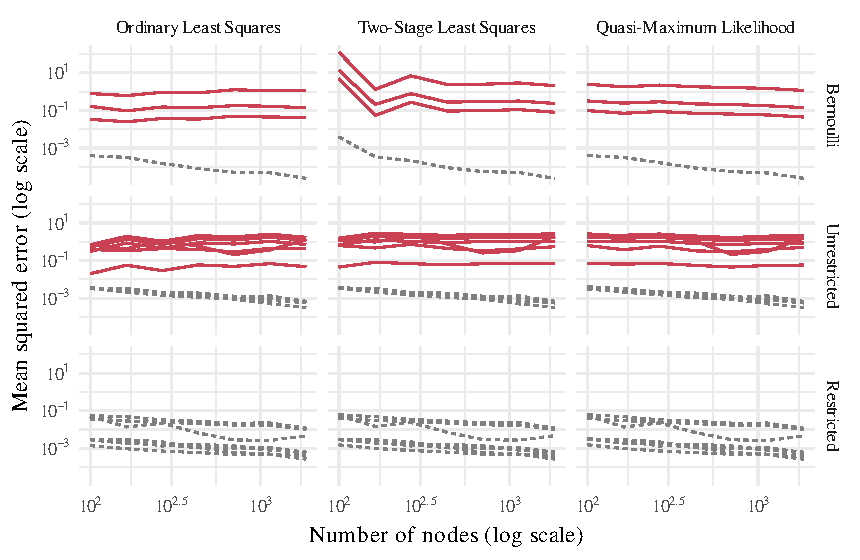
\includegraphics[width=0.9\textwidth]{./figures/simulations/biometrika-mse-all.pdf}
                    \caption{\textcolor{Mahogany}{Red lines} represent estimation error for asymptotically aliased regression coefficients, and \textcolor{gray}{gray lines} represent estimation error for asymptotically un-aliased coefficients.}
                \end{figure}

            \end{block}

            \begin{block}{Takeaways}
                \begin{enumerate}
                    \item It can be impossible to estimate peer effects using linear-in-means models, even when all parameters in the model are identified. This is primarily an issue for Bernoulli designs in dense networks, or under models with growing minimum degree.
                    \item In observational data from random dot product models (like stochastic blockmodels), it may be possible to avoid colinearity issues by including latent network structure in the regression
                    \item In controlled experiments, use network-specific designs like graph-cluster or ego-cluster randomization to avoid colinearity issues
                \end{enumerate}
            \end{block}

            \begin{block}{Want to learn more? Have a comment? Pre-print \& contact info}
                \nocite{hayes2024c}
                \printbibliography


                \begin{columns}
                    \begin{column}{0.4\textwidth}
                        \begin{center}
                            \url{alex.hayes@wisc.edu} \\
                            \url{https://www.alexpghayes.com}
                        \end{center}
                    \end{column}
                    \begin{column}{0.3\textwidth}
                        \begin{figure}
                            \centering
                            
\includegraphics[width=0.45\textwidth]{./figures/arxiv-qr.png}
                        \end{figure}
                    \end{column}
                \end{columns}
            \end{block}
        \end{column}
        \separatorcolumn
    \end{columns}
\end{frame}

\end{document}
